% \documentclass{article}
% \usepackage[utf8]{inputenc}

% \title{MO444}
% \author{lucasrm25 }
% \date{March 2018}

% \begin{document}

% \maketitle

% \section{Introduction}

% what assays 

% \end{document}



%%% PREAMBLE - Do not touch %%%%%%%%%%%%%%%%%%%%%%%%%%%%%%%%%%%%%%%%%%%%%%%%%%%%%%
\documentclass[10pt,twocolumn,letterpaper]{article}
\usepackage[ansinew]{inputenc}
\usepackage[portuges,brazil,english]{babel}
\usepackage{model}
\usepackage{times}
\usepackage{epsfig}
\usepackage{graphicx}
\usepackage{amsmath}
\usepackage{amssymb}
\usepackage{color}
\usepackage[pagebackref=true,breaklinks=true,letterpaper=true,colorlinks,bookmarks=false]{hyperref}
\input{pics/abaco}

\cvprfinalcopy % *** Uncomment this line for the final submission
\def\httilde{\mbox{\tt\raisebox{-.5ex}{\symbol{126}}}}
\ifcvprfinal\pagestyle{empty}\fi

\newcommand{\TODO}[1]{TODO: #1}
\newcommand{\CITEONE}[2]{\mbox{#1 \cite{#2}}}
\newcommand{\CITETWO}[3]{\mbox{#1 and #2 \cite{#3}}}
\newcommand{\CITEN}[2]{\mbox{#1 et al. \cite{#2}}}

%%% Report beginning %%%%%%%%%%%%%%%%%%%%%%%%%%%%%%%%%%%%%%%%%%%%%%%%%%%%%%%%%%%%%%
\begin{document}



%%% Title and authors %%%%%%%%%%%%%%%%%%%%%%%%%%%%%%%%%%%%%%%%%%%%%%%%%%%%%%%%%%%%
\title{A GA-trained NN-based Control Method for Autonomous Vehicles}
\author{Gustavo Ciotto Pinton\thanks{Is with the Institute of Computing, University of Campinas (Unicamp). \textbf{Contact}: \tt\small{gustavociotto@gmail.com}}\\
Lucas Rath Maia\thanks{Is with the Faculty of Mechanical Engineering, University of Campinas (Unicamp). \textbf{Contact}: \tt\small{lucasrm25@gmail.com}}
}



%%% Abstract %%%%%%%%%%%%%%%%%%%%%%%%%%%%%%%%%%%%%%%%%%%%%%%%%%%%%%%%%%%%%%%%%%%%%
\maketitle
\begin{abstract}
In this report, the authors present the main motivations that led them to choose this subject as the final project for the Pattern Recognition and Machine Learning course. A brief analysis of previous works in the subject and the expected results are also presented.
\end{abstract}



%%% Introduction %%%%%%%%%%%%%%%%%%%%%%%%%%%%%%%%%%%%%%%%%%%%%%%%%%%%%%%%%%%%%%%%%
\section{Introduction}

Improvements in processing power in the last few years together with a big offer of available data have made possible many problems be approached with machine learning-related techniques. Among these problems, the control of autonomous vehicles stands out for its great financial attractiveness as many major market players, such as BMW, Tesla and Mercedes invest a lot of resources in this branch of technology \cite{News}. Having considering those facts, we propose a method to control of autonomous vehicles based on neural networks, whose training is performed by an evolutionary algorithm. Here, the goal is that a self-driven vehicle learns how to drive autonomously an specific race track in less time as possible based only on sensors placed on the simulated vehicle. 

In it's simplest implementation, the proposed model will be modeled based on states, actions and rewards possible in the environment. The states are considered to be the environment sensing, such as, vehicle's speed, acceleration, angular velocity and five inputs produced by sensors that will measure the distance of the simulated object to the walls at different angular directions. Next, the actions are consisted by all the possible actions that the autonomous driver can take facing an specific state every moment. Consequently, actions are the composed by the actuation of the accelerating and brake pedal and also the steering wheel angle. Finally, each autonomous-driver model will be rewarded and ranked based on how good the vehicle can be self-driven during the race track, i.e. how far the vehicle can drive without hitting any wall and in the case the vehicle completes one lap, how fast it can drive.

Therefore, this paper will explore different neural network structures and evolutionary learning strategies in order to maximize the vehicle self-driveability performance.

%The main goal of this work is, therefore, to evaluate the impact of different parameters (layers size, mutation ratio, fitness function etc) on the control quality.

%The proposed model will consider some real life features, such as, vehicle's speed and acceleration and inputs produced by five sensors placed in the sides, front and back of the simulated object. The main goal of this work is, therefore, to evaluate the impact of different parameters (layers size, mutation ratio, fitness function etc) on the control quality.

%Here goes the introduction and motivation of the work.
%
%Some directions for the paper:
%
%\begin{itemize}
%	\item Diagrams and figures are encouraged for making the paper richer
%	\item The sections proposed here are not hard-constrained. It means, you 
%	can propose other sections as well as change the existing ones. 
%\end{itemize}



%%% Add section %%%%%%%%%%%%%%%%%%%%%%%%%%%%%%%%%%%%%%%%%%%%%%%%%%%%%%%%%%%%%%%%%%
\section{Activities}

Some articles have already discussed how to use a genetic algorithm to train neural networks in order to provide control for autonomous systems, notably \cite{8102147}, \cite {SALOMON1997199} and \cite {6146976}. In the final report, the solutions presented by their authors will be discussed and compared with the one we proposed.

% Here goes the state-of-the-art research (talk about prior work for solving the same problem). We need to cite the article we found.


%%% Add section %%%%%%%%%%%%%%%%%%%%%%%%%%%%%%%%%%%%%%%%%%%%%%%%%%%%%%%%%%%%%%%%%%
\section{Proposed Solutions}

Given one or more training maps, such as the one in the figure \ref{fig:roadMap}, we propose to train a neural network capable of controlling a vehicle in any other map. The chosen training maps must be sufficiently good to represent the biggest number of real life situations commonly found in any other track, otherwise the neural network resulted from this training might not know how to proceed in unknown states. It should be noted that the GA parameter settings must also take into account the bad effects of over fitting. 

\begin{figure}
    \centering
    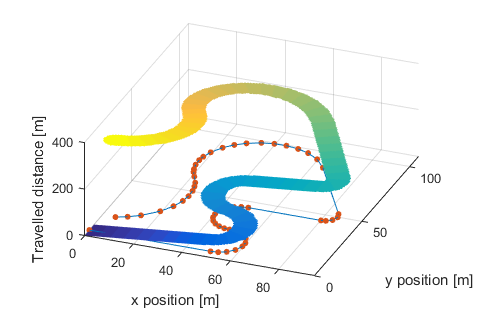
\includegraphics[width=0.89\columnwidth]{roadMap.png}
    \caption{Road map}
    \label{fig:roadMap}
\end{figure}

For the start, the proposed neural network receives 7 inputs states - vehicle's speed, acceleration, angular velocity and 5 distance sensors - and produces 3 outputs actions - a new steering angle and a brake and acceleration pedal actuation. The genetic algorithm, generations with \(i = 1000\) individuals are submit to the training maps and evaluated according to the fitness function which considers the time and distance that the simulated object took during the simulation. Eventual collisions are evidently penalized.

% \begin{equation}
%     \label{eq:fitness}
%     F(x) = ....
% \end{equation}



%%% Add section %%%%%%%%%%%%%%%%%%%%%%%%%%%%%%%%%%%%%%%%%%%%%%%%%%%%%%%%%%%%%%%%%%
%\section{Experiments and Discussion}
% Talk about the experiments carried out and the obtained results. 

% Examples of citations~\cite{Ni_2008, Ni_2009}. For direct citations use something like: 

% \CITEONE{Silva}{Silva_2010} for papers with one author.
% \CITETWO{Silva}{Souza}{Silva_2010b} for papers with two authors.
% \CITEN{Silva}{Silva_2010c} for papers with three or more authors.

% Example of a figure of one column. 
% \begin{figure}
% \begin{center}
% 	\includegraphics[width=0.99\columnwidth]{pics/example-figure}
% 	\caption{A figure example spanning one column only.\label{fig:label}}   
% \end{center} 
% \end{figure}   

% Example of a figure spanning two columns. 
% \begin{figure*}
% \begin{center}
% 	\includegraphics[width=0.99\textwidth]{pics/example-figure-spanned}
% 	\caption{A figure example spanning two columns.\label{fig:label2}}   
% \end{center} 
% \end{figure*}

% Example of a table spanning only one column: 

% \begin{table}
% \begin{center}
% \begin{tabular}{l*{6}{c}r}
% Team              & P & W & D & L & F  & A & Pts \\
% \hline
% Manchester United & 6 & 4 & 0 & 2 & 10 & 5 & 12  \\
% Celtic            & 6 & 3 & 0 & 3 &  8 & 9 &  9  \\
% Benfica           & 6 & 2 & 1 & 3 &  7 & 8 &  7  \\
% FC Copenhagen     & 6 & 2 & 1 & 2 &  5 & 8 &  7  \\
% \end{tabular}
% \end{center}
% \end{table}

% Example of a table spanning two columns: 

% \begin{table*}
% \begin{center}
%     \begin{tabular}{ | l | l | l | p{8cm} |}
%     \hline
%     Day & Min Temp & Max Temp & Summary \\ \hline
%     Monday & 11C & 22C & A clear day with lots of sunshine.  
%     However, the strong breeze will bring down the temperatures. \\ \hline
%     Tuesday & 9C & 19C & Cloudy with rain, across many northern regions. Clear spells
%     across most of Scotland and Northern Ireland,
%     but rain reaching the far northwest. \\ \hline
%     Wednesday & 10C & 21C & Rain will still linger for the morning.
%     Conditions will improve by early afternoon and continue
%     throughout the evening. \\
%     \hline
%     \end{tabular}
% \end{center}    
% \end{table*}



%%% Add section %%%%%%%%%%%%%%%%%%%%%%%%%%%%%%%%%%%%%%%%%%%%%%%%%%%%%%%%%%%%%%%%%%
%\section {Conclusions and Future Work}

%Although many approaches, such as reinforced learning, are possible when talking about autonomous cars control we have presented in the previous sections some previous works which were based on the same concepts and techniques that we intend to use in our project. For the first part, we will design a map with realist contour situations and evaluate the genetic algorithm's evolution parameters that will determine the synaptic weights of the neural network neurons. The next step is to evaluate if the generated neural network presents positive results for random new maps.

% Present the main conclusions of the work as well as some future directions for other people interested in continuing this work. 

% "In addition, solutions that are successful in one mission environment may not be desirable in another mission. This section briefly discusses these challenges and techniques to overcome them." Multi-Layer Model of Swarm 



%%% References %%%%%%%%%%%%%%%%%%%%%%%%%%%%%%%%%%%%%%%%%%%%%%%%%%%%%%%%%%%%%%%%%%%
{\small
\bibliographystyle{unsrt}
\bibliography{refs}
}

\end{document}